\documentclass[12pt,letterpaper]{article}
\usepackage[margin=1in]{geometry}
\usepackage{fancyhdr}
\usepackage[utf8]{inputenc}
\usepackage{palatino}
\usepackage{microtype}
\usepackage{hyperref}
\usepackage{graphicx}
\usepackage{lastpage}
\usepackage[hang,small]{caption}
\usepackage{titlesec}
\usepackage{amsmath,amssymb}
\usepackage{multirow}

\renewcommand{\headrulewidth}{0pt}
\fancyfoot{}
\fancyfoot[C]{\sf Page \thepage\ of \pageref{LastPage}}
\pagestyle{fancy}

\titleformat{\section}{\bfseries\Large}{\arabic{\thesection}}{1em}{}
\titleformat{\subsection}{\bfseries\large}{\arabic{\thesection}.\arabic{\thesubsection}}{1em}{}
\titleformat{\subsubsection}{\itshape}{\arabic{\thesection}.\arabic{\thesubsection}.\arabic{\thesubsubsection}}{1em}{}

\setlength{\parindent}{0cm}
\setlength{\parskip}{0.8em}

\captionsetup[figure]{labelfont=it,font=it}
\captionsetup[table]{labelfont={it,sc},font={it,sc}}

\hypersetup{colorlinks,
    linkcolor = black,
    citecolor = black,
    urlcolor  = black}
\urlstyle{same}



\begin{document}

Soo-Hyun Yoo \\
ST314 \\
Data Analysis 2\\
October 21, 2014

\begin{enumerate}
	\item \hfill\\
		\begin{table}[!h]
			\centering
			\begin{tabular}{|c|c|c|} \hline
				Dis. Dist. & Binomial & Poisson \\ \hline\hline
				pmf & $\left(^n_k\right) p^k(1-p)^{n-k}$ & $\frac{\lambda^k}{k!}e^{-\lambda}$ \\ \hline
				$E(x)$ & $np$ & $\lambda$ \\ \hline
				$V(x)$ & $np(1-p)$ & $\lambda$ \\ \hline
			\end{tabular}
		\end{table}
		\begin{table}[!h]
			\centering
			\begin{tabular}{|c|c|c|c|} \hline
				Con. Dist. & Uniform & Exponential & Gamma \\ \hline\hline
				pdf & $\frac{1}{b-a}$ & $\lambda e^{-\lambda x}$ &  \\ \hline
				$E(x)$ & $\frac{a+b}{2}$ & $\frac{1}{\lambda}$ & \\ \hline
				$V(x)$ & $\frac{(b-a)^2}{12}$ & $\frac{1}{\lambda^2}$ & \\ \hline
			\end{tabular}
		\end{table}
	\item
		\begin{enumerate}
			\item \hfill\\ 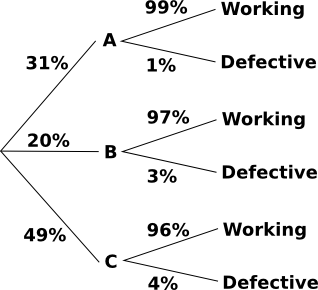
\includegraphics[width=0.5\textwidth]{2a.png}
			\item $0.31 \cdot 0.01 + 0.20 \cdot 0.03 + 0.49 \cdot 0.04 = \boxed{0.0287}$
			\item $\cfrac{0.49 \cdot 0.04}{0.0287} = \boxed{0.683}$
		\end{enumerate}

	\item 
		\begin{enumerate}
			\item If $f$ is to be a legitimate pdf, its integral from 0 to
				$\infty$ must equal 1. With $u = 1+\frac{x}{3}$,
				\begin{align*}
					\int_0^\infty c\left(1+\frac{x}{3}\right)^{-4} \;dx &= 1 \\
					3c\int_0^\infty u^{-4} \;du &= 1 \\
					3c\left.\left(-\frac{1}{3}\right)u^{-3} \right|_0^\infty &= 1 \\
					-c\left.\left(1+\frac{x}{3}\right)^{-3} \right|_0^\infty &= 1 \\
					0 - (-c\cdot1) &= 1 \\
					c &= \boxed{1}.
				\end{align*}
			\item $1000\int_0^\infty x\left(1+\frac{x}{3}\right)^{-4} \;dx = \boxed{\$1500}$
			\item $1000\sqrt{\int_0^\infty (x-1.5)^2 \left(1+\frac{x}{3}\right)^{-2} \;dx} = \boxed{\$2598}$
			\item $1500 + 1.645\cdot2598 = \boxed{\$5774}$
			\item $0.90 \cdot 1500 = \boxed{\$1350}$
		\end{enumerate}

	\item 
		\begin{enumerate}
			\item $E(x) = \frac{1}{\lambda} = 2000$, so $\lambda = \frac{1}{2000}$. Then the cdf $F(x) = \boxed{1-e^{-\frac{x}{2000}}}$.
			\item Solving $F(x) = 0.5$ gives $x = 1386$. The exponential distribution is skewed right, so the median is less than the mean.
			\item $1-F(2100) = \boxed{0.350}$
			\item $(1-F(2100))^6(F(2100)) * 7 + (1-F(2100))^7 = \boxed{0.00900}$
		\end{enumerate}

	\item 
		\begin{enumerate}
			\item \hfill\\ 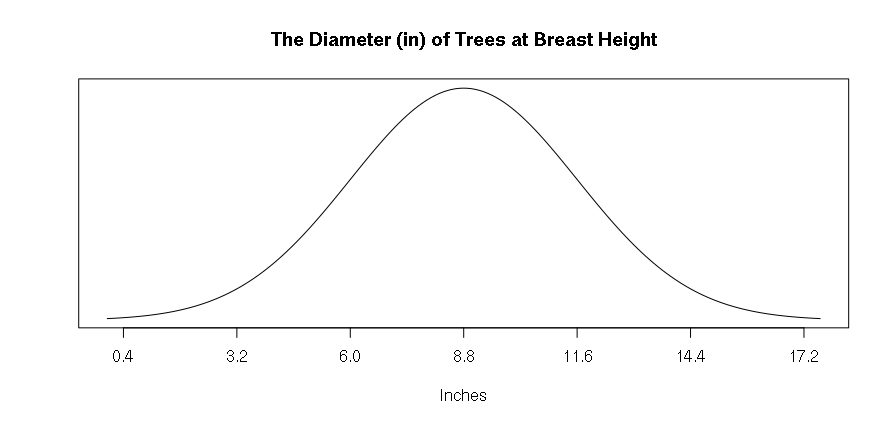
\includegraphics[width=0.8\textwidth]{5a.png}
			\item 9 is $\frac{9-8.8}{2.8} = 0.0714\sigma$ away from the mean.
				The z-score is then $\boxed{0.4715}$.
			\item 7 is $\frac{7-8.8}{2.8} = -0.643\sigma$ away from the mean.
				The z-score here is $0.7398$. The probability of the diameter
				of a randomly selected tree being between 7 and 9 inches is
				then $0.7398 - 0.4715 = \boxed{0.2683}$.
			\item The z-score is $0.05$ at $\sigma = 1.645$. Then $c = 1.645 \cdot 2.8 = \boxed{4.606}$.
			\item
				\begin{verbatim}
				> 1 - pnorm(9, 8.8,2.8)
				[1] 0.4715283
				> pnorm(9, 8.8,2.8)-pnorm(7, 8.8,2.8)
				[1] 0.2683133
				> c = 8.8 - qnorm(.05,8.8,2.8) # or qnorm(.95,8.8,2.8) - 8.8
				> c 
				[1] 4.60559
				> check = pnorm(8.8+c, 8.8,2.8)-pnorm(8.8-c,8.8,2.8)
				> check
				[1] 0.9
				\end{verbatim}
		\end{enumerate}
\end{enumerate}

\end{document}

